
\begin{frame}{Phänomenologie}
\textbf{Supraleitung}: Ab einer Sprungtemperatur $T_{\mathup{C}}$ fällt elektrischer Widerstand auf $\SI{0}{\ohm}$ \\
\begin{columns}
\begin{column}{0.49\textwidth}
  \begin{figure}
    \fbox{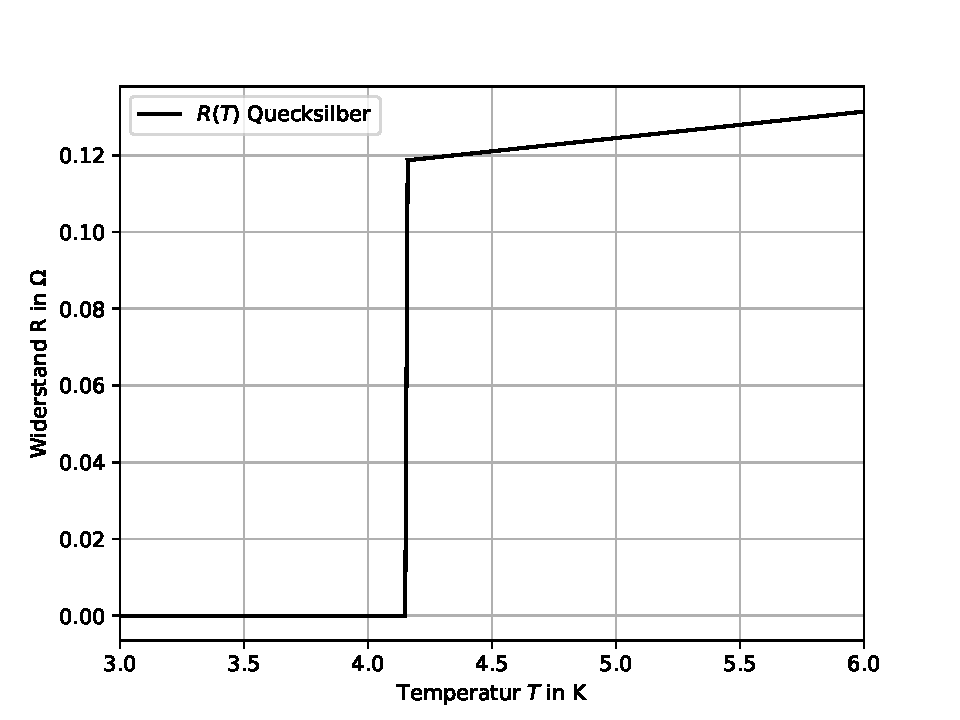
\includegraphics[width = \textwidth]{bilder/quecksilber_supra.pdf}}
    \label{fig: hg_supraleitung}
  \end{figure}
\end{column}
\begin{column}{0.49\textwidth}

\begin{table}
  \caption{Sprungtemperaturen \cite{dem2}}
  \label{tab: sprungtemperaturen}
\begin{tabular}{l S}
  & $T_{\mathup{C}} / \si{\kelvin}$ \\
  \text{Quecksilber} & \num{4.15} \\
    \text{Aluminium} & \num{1.17} \\
      \text{\ce{TlCaBaCuO}} & \num{125}
\end{tabular}
\end{table}
\pause
\begin{itemize}
  \item Hochtemperatur-Supraleiter für Versuch geeignet
\end{itemize}

\end{column}
\end{columns}
\end{frame}


\section{Theorie}
\begin{frame}{Meißner-Ochsenfeld-Effekt}
\begin{columns}
\begin{column}{0.49\textwidth}
  \begin{figure}
    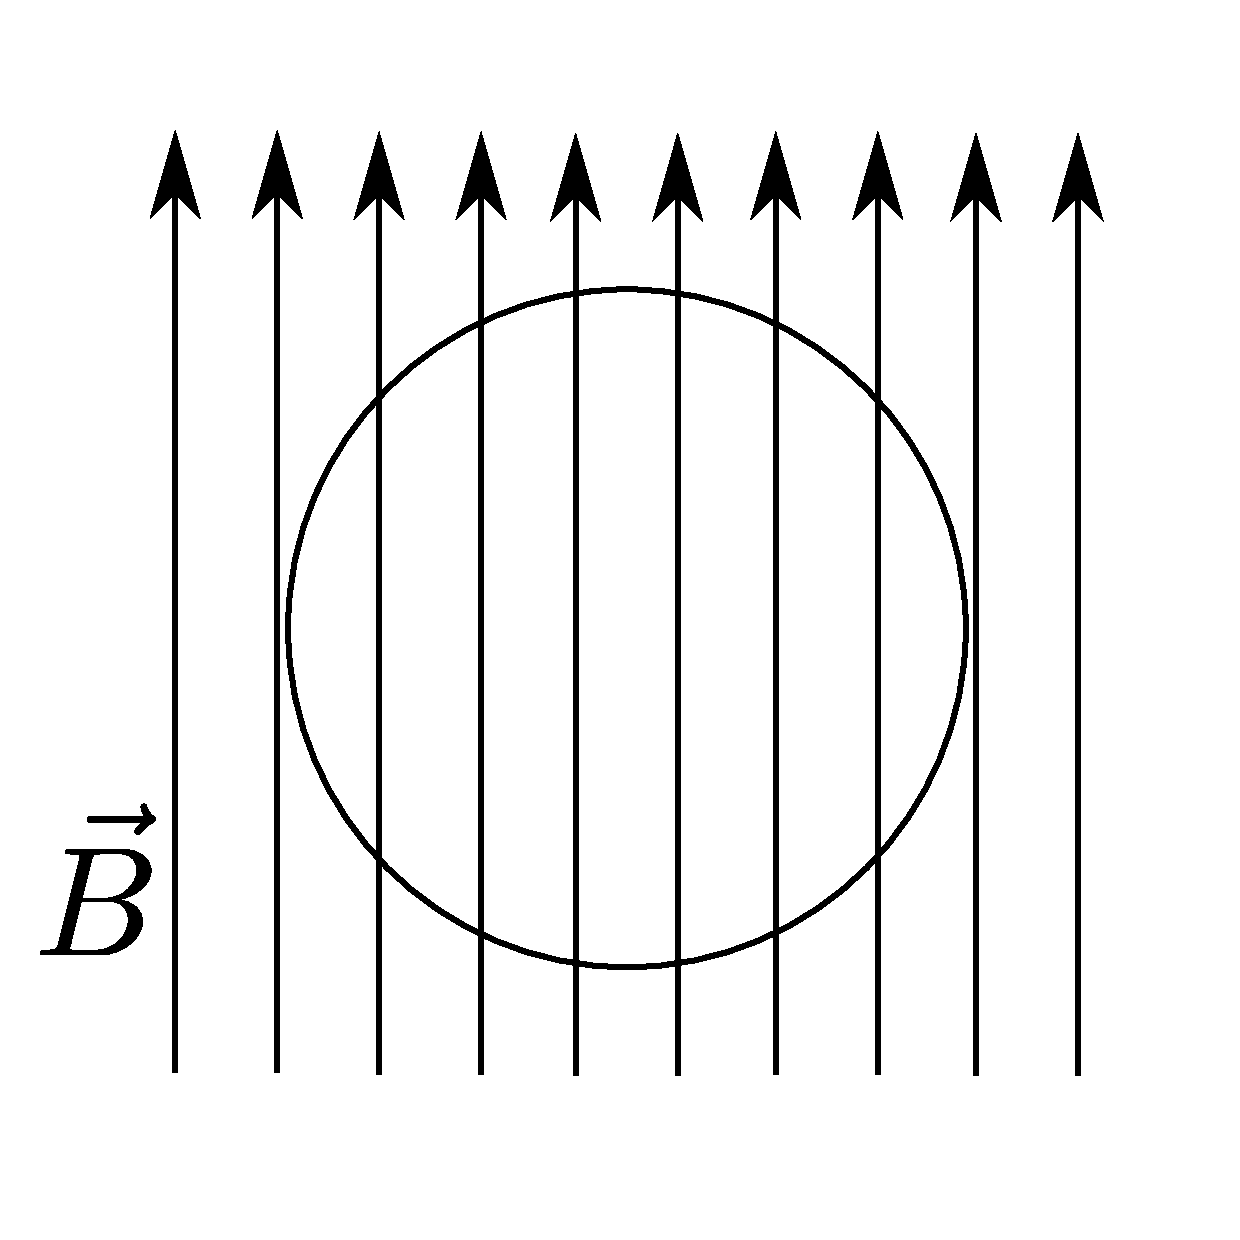
\includegraphics[width = \textwidth]{bilder/supra_1.pdf}
    \caption{Normale Leitung $T > T_{C}$}
    \label{fig: bfeld_normale_leitung}
  \end{figure}
\end{column}
\begin{column}{0.49\textwidth}
  \begin{figure}
    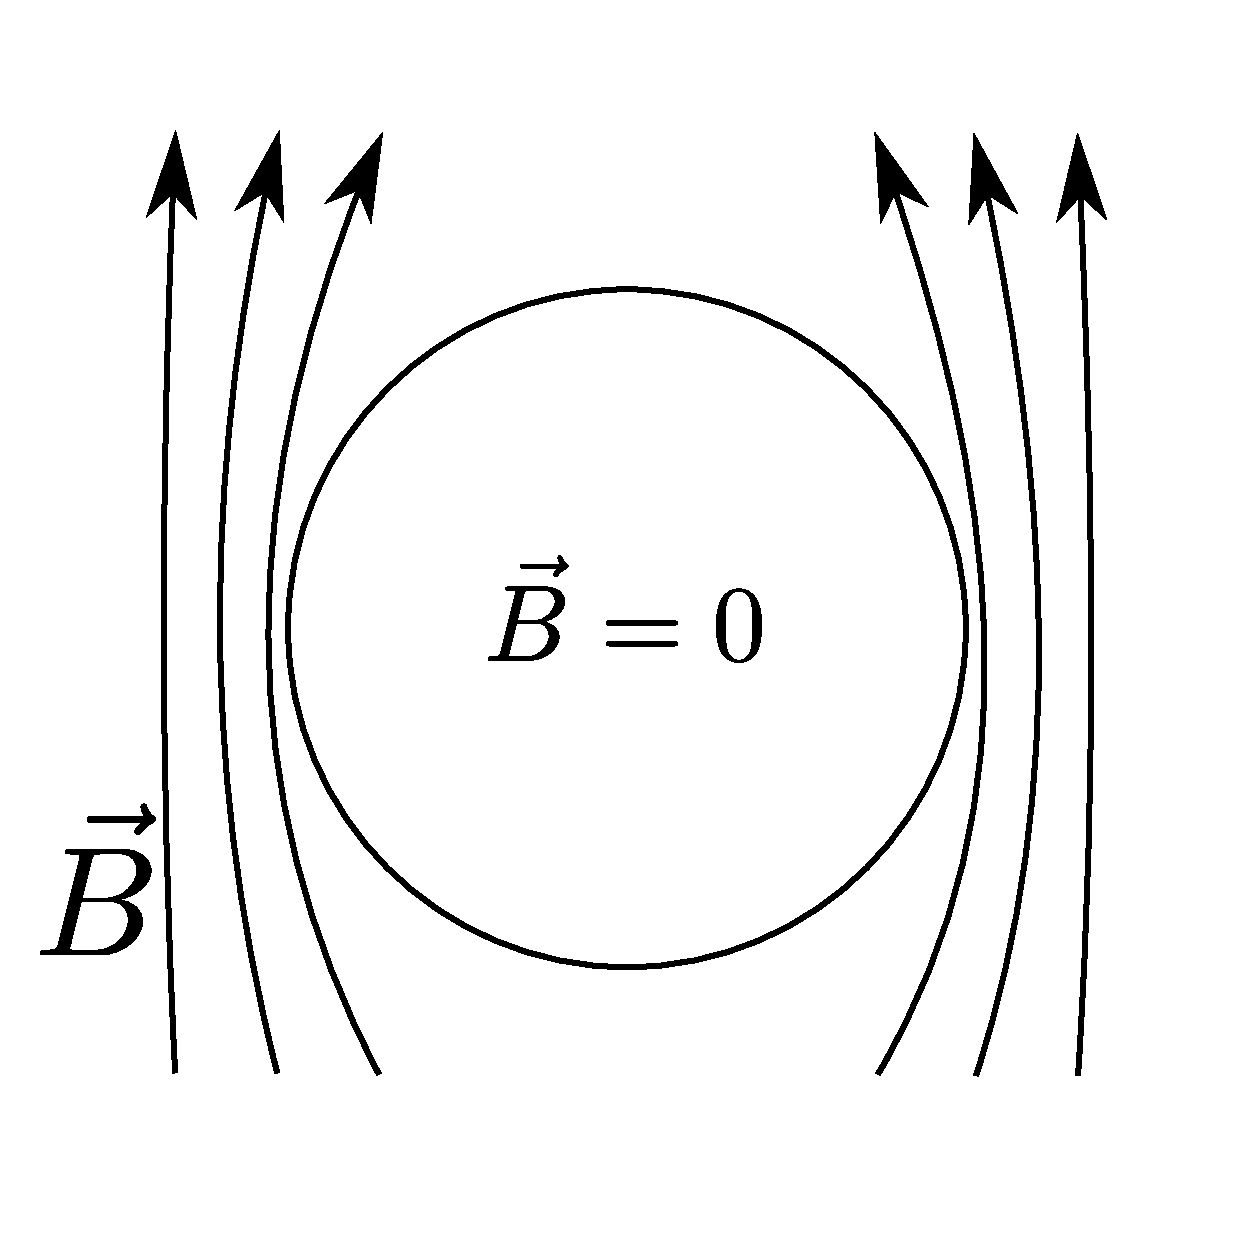
\includegraphics[width = \textwidth]{bilder/supra_2.pdf}
    \caption{Supraleitung $T < T_{C}$}
    \label{fig: bfeld_supraleitung}
  \end{figure}
\end{column}
\end{columns}
\end{frame}

\begin{frame}{Eigenschaften}
  \begin{enumerate}
    \item idealer Leiter $R = 0$
    \item idealer Diamagnet (Suszeptibilität $\chi = -1$)
    \begin{equation*}
      \vec{M} = \chi \vec{H} \quad \Rightarrow \quad \vec{B} = \mu_0 (\vec{H} + \vec{M}) = 0
    \end{equation*}
    Kein Magnetfeld im Inneren des Supraleiters
  \end{enumerate}

\end{frame}
\begin{frame}{Quantitative Beschreibung}
Londongleichungen ersetzen das ohmsche Gesetz
\begin{equation*}
  \vec{\jmath} = \frac{\tau n q^2}{m}\cdot \vec{E} = \sigma\cdot \vec{E}\quad  \longrightarrow \quad
  \begin{cases}
    \frac{\partial }{\partial t}\vec{\jmath} &= \frac{nq^2}{m}\vec{E} \\
    \nabla \times \vec{\jmath} &= - \frac{n q^2}{m} \vec{B}
  \end{cases}
\end{equation*}
\pause
Mit Maxwell Gleichung $\nabla \times \vec{B} = \mu_0 \vec{\jmath}$
\begin{equation*}
-\nabla \times (\nabla \times \vec{B}) = -\nabla\underbrace{(\nabla \cdot \vec{B})}_{= 0} + \Delta \vec{B}
\end{equation*}
\begin{equation*}
\Rightarrow  \Delta \vec{B} = \frac{\mu_0 n q^2}{m}\vec{B}
\end{equation*}
\end{frame}

\begin{frame}{Quantitative Beschreibung}

\begin{columns}
\begin{column}{0.49\textwidth}
\begin{align*}
    \text{Ansatz:} \quad \vec{B}_i &= (0, 0, B_z(x))^T \\
  \Rightarrow \frac{\partial ^2}{\partial x^2}B_z &= \frac{1}{\lambda ^2}B_z, \quad \lambda = \sqrt{\frac{m}{\mu_0 n q^2}}
\end{align*}
(sinnvolle) Lösung:
\begin{align*}
   \vec{B} &= B_0 \exp\left[-\frac{x}{\lambda}\right]\vec{e}_z \\
   \Rightarrow \vec{\jmath} &= \frac{B_0}{\mu_0 \lambda}\exp \left[-\frac{x}{\lambda} \right] \vec{e}_y
\end{align*}
Eindringtiefe $\lambda$, Größenordnung $\SI{100}{\nano\meter}$
\end{column}
\begin{column}{0.49\textwidth}
  \begin{figure}
    \centering
    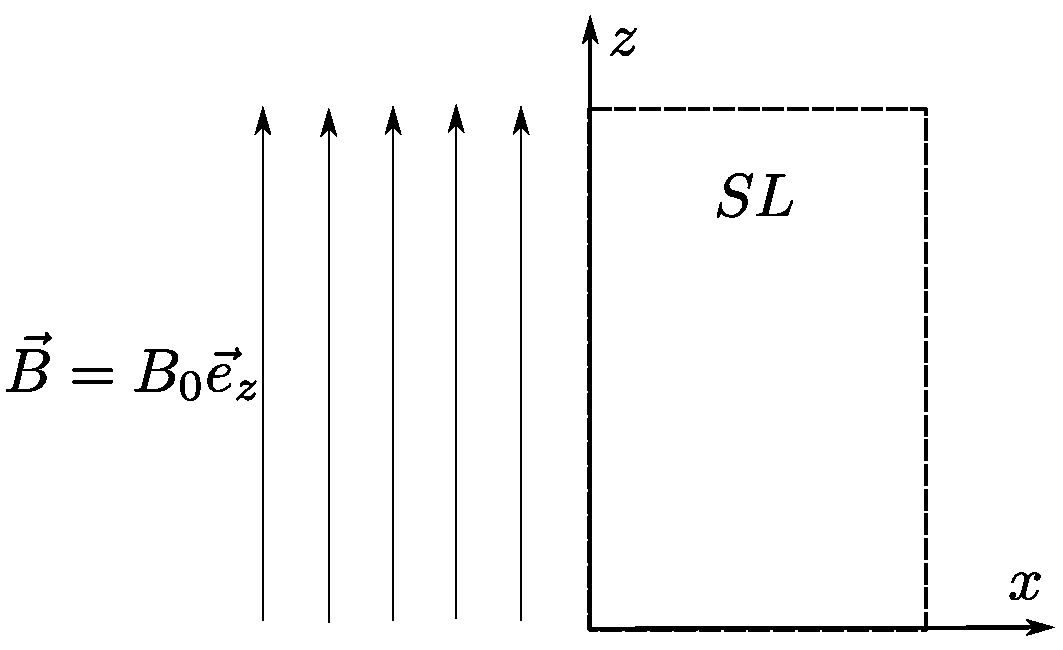
\includegraphics[width = 0.7\textwidth]{bilder/supra_3.pdf}
    \label{fig: londongleichungen}
  \end{figure}
  \pause
  \begin{figure}
    \centering
    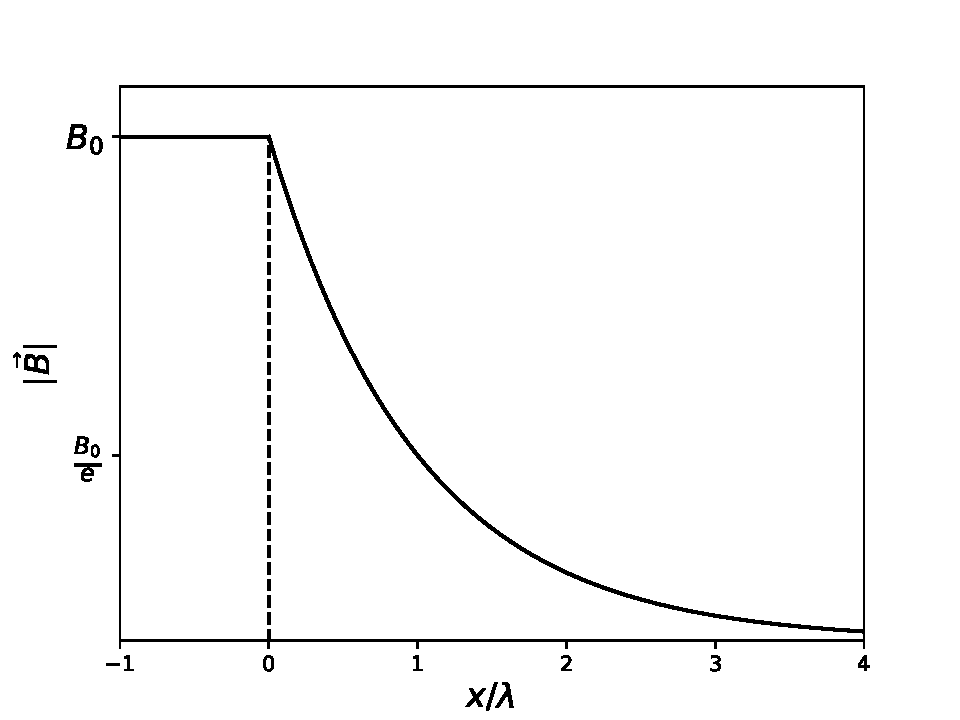
\includegraphics[width = 0.9\textwidth]{bilder/plot_london.pdf}
    \label{fig: plot_londongleichungen}
  \end{figure}
\end{column}
\end{columns}

\end{frame}


\begin{frame}{Was sind die Träger des Suprastroms?}
  \begin{figure}
    \centering
    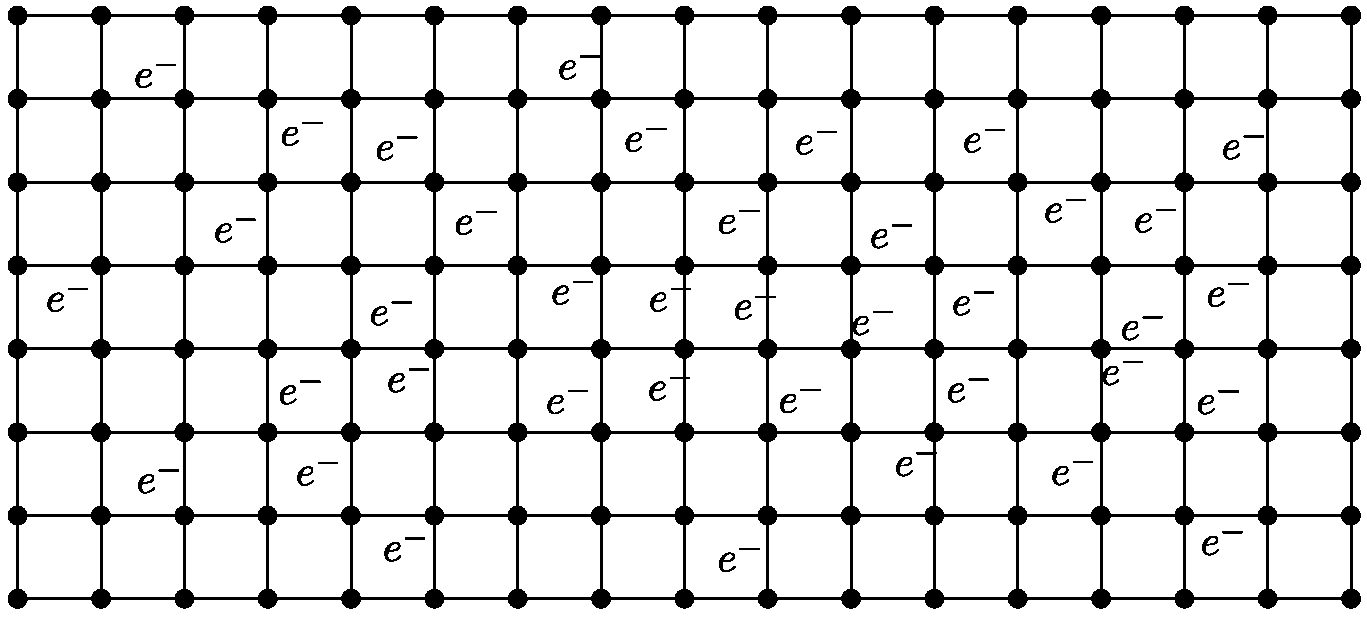
\includegraphics[width = 0.9\textwidth]{bilder/elektronengas.pdf}
    \label{fig: elektronengas}
  \end{figure}
\end{frame}


\begin{frame}{Cooper-Paare}
  \begin{figure}
    \centering
    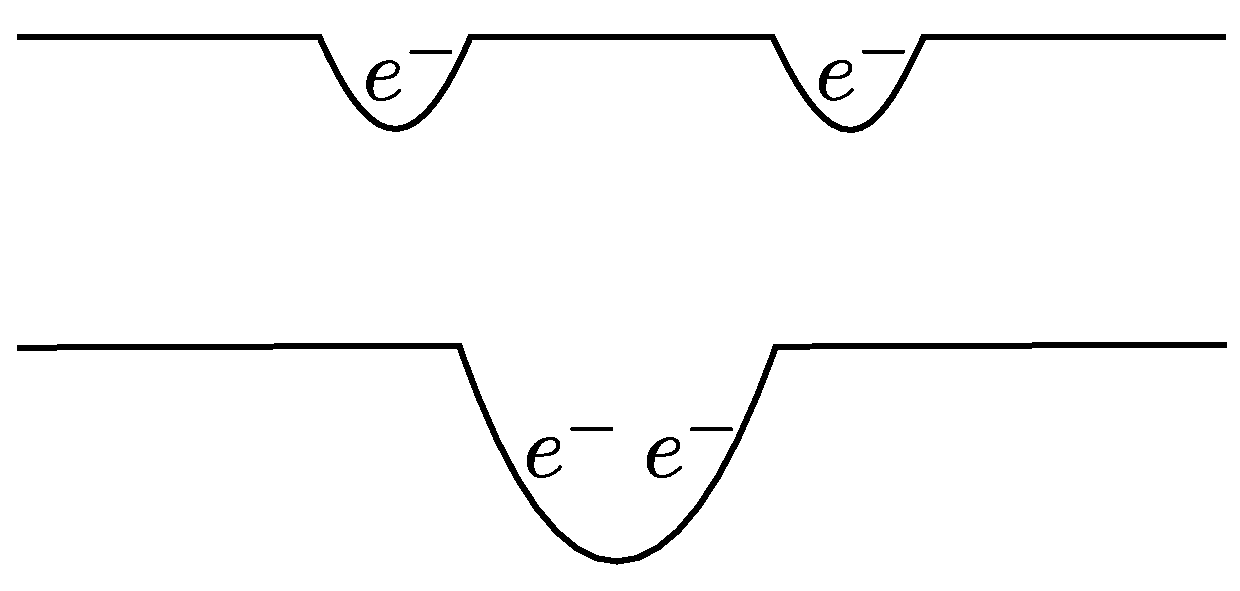
\includegraphics[width = 0.9\textwidth]{bilder/cooper.pdf}
    \label{fig: cooper}
  \end{figure}
\end{frame}
